\section{\tool}
\label{sec:tool}

\subsection{Goals}
\label{sec:tool:goals}

We identify the broad design goals for a technique to automatically repair
malformed strings or incorrect handling of strings as follows:

% i) identifies the statements which might be vulnerable to string-related errors,
% and are less critical to the functionality of the application such that
% suboptimal behavior might be acceptable,
% iii) generates patches by identifying constraints on the string data and if
% required, tweaks \code{String} API  parameters to regenerate legally correct
% string data,
% iv) optimizes the number of statements to be patched by retaining only the ones
% that need to be protected,  

\myparagraph{(i) High patch fidelity} We require that the patched program must
preserve the intended program behavior, \ie\ the patch must be precise, and
should not induce any undesirable control flows in the repaired program.

\myparagraph{(ii) Non-invasive instrumentation} We require that the technique
must ensure no side-effects (aside from optimally repairing objects) during
normal program execution, and activate patches only when the program is
guaranteed to crash.

\myparagraph{(iii) Low system overhead} We desire that the patched program must
incur no runtime overhead during normal program execution, and only negligible
overhead in case of failures.

\subsection{Design}
\label{sec:tool:design}

\begin{figure}[t]
\centering
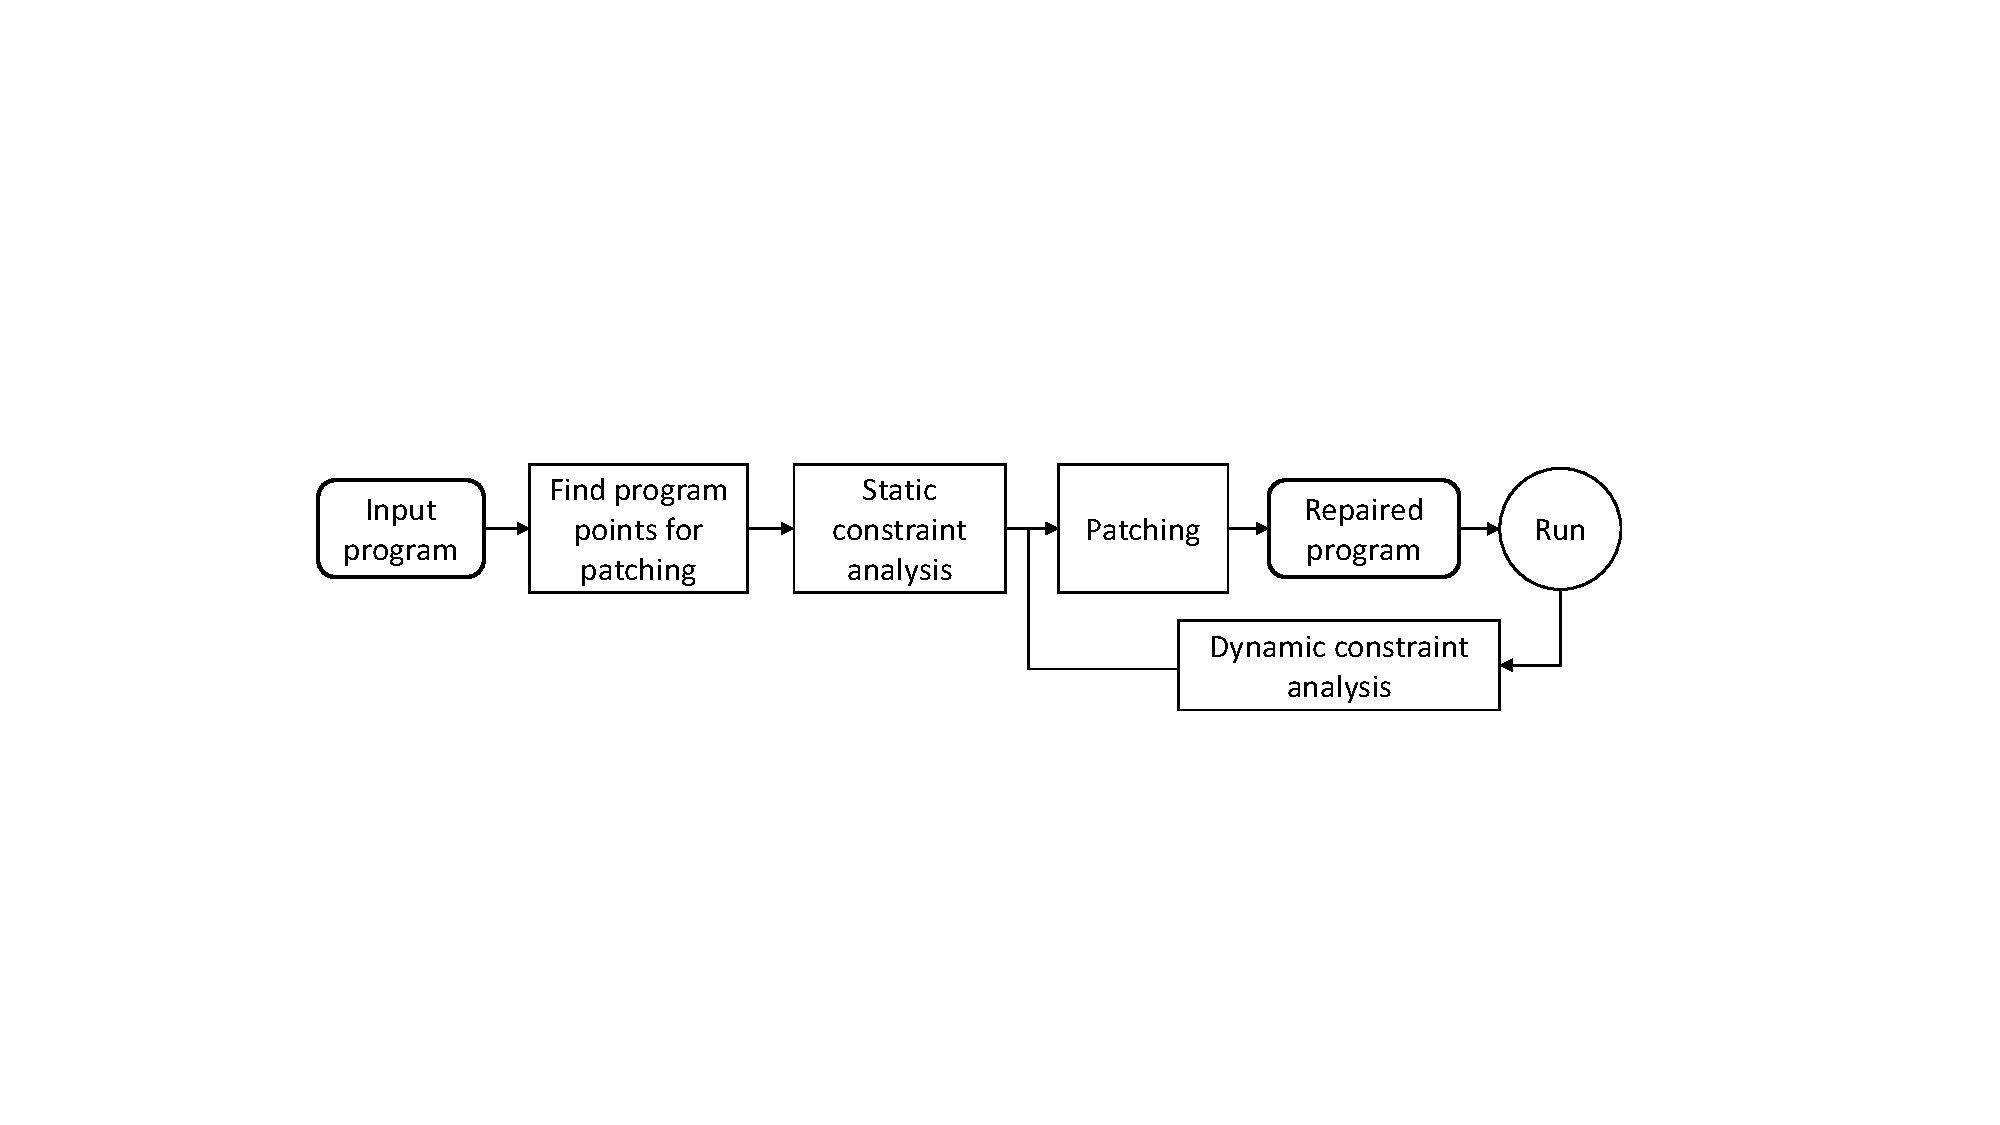
\includegraphics[scale=.38]{images/NewDesignDiagram.pdf}
\caption{\tool\ workflow.}
\label{fig:overallDesign}
\end{figure}

\myparagraph{\underline{Key Idea}} \tool\ leverages precise taint analysis and
call graph analysis to identify program instrumentation points, and builds upon
custom algorithms to generate targeted, high quality patches for repairing
programs with potential runtime exceptions, while still satisfying goals
mentioned in \xref{sec:tool:goals}.

Figure~\ref{fig:overallDesign} shows \tool's workflow, which involves three
main stages. First, \tool\ uses precise program analysis techniques to identify
points of interest, \ie\ string objects or API arguments that must be repaired
to prevent runtime exceptions. In the second stage, \tool\ leverages custom
algorithms to generate relevant patches. Specifically, \tool\ performs
intra-procedural static and dynamic analyses to identify and evaluate
constraints on the string objects under consideration. Third, \tool\ uses the
constraints evaluated in the earlier stage to programatically generate and embed
patches inside \texttt{catch} blocks to ensure that they do not get activated
during normal program execution.

\subsubsection{Precise Identification of Instrumentation Points}
\label{sec:tool:stage1}

In this stage, \tool\ leverages a combination of program analyses to accurately
determine the minimum set of points of interest where instrumentation is
required to repair. We list several techniques below that help \tool\ achieve
precision.

\myparagraph{(i) Taint analysis}: The main purpose of taint analysis is to
broadly identify which program statements can be patched (possibly even
suboptimally) without affecting the program control flow, \ie\ affect only
objects that are generated and stay within the application throughout their
lifetime. While this principle is not a binding constraint, it ensures that
\tool's repairing mechanism does not adversely affect critical program behavior.
We specify a generic set of sensitive sources and sensitive sinks for each input
program, to identify critical program paths where a repaired \code{String}
objects (and thus possibly suboptimal) must not flow. For example, \tool\ does
not repair program statements that lie along a control flow path that leads to
an I/O sink, like file system, console, network, GUI, etc.

\begin{table}[t]
\centering
\scriptsize
% \setlength{\tabcolsep}{3pt}
\begin{tabular}{l|l}
\multicolumn{1}{c|}{\textbf{Class}} & \multicolumn{1}{c}{\textbf{Source}}\\
\hline
\code{java.io.InputStream} & \code{read()}\\
\code{java.io.BufferedReader} & \code{readLine()}\\
\code{java.net.URL} & \code{openConnection()}\\
\code{java.util.Scanner} & \code{next()}\\
% \code{javax.servlet.http.HttpServletRequest} & \code{getParameter()}\\
\code{javax.servlet.ServletRequest} & \code{getParameter()}\\
\code{org.apache.http.HttpResponse} & \code{getEntity()}\\
\code{org.apache.http.util.EntityUtils} & \code{toString()}\\
\code{org.apache.http.util.EntityUtils} & \code{toByteArray()}\\
\code{org.apache.http.util.EntityUtils} & \code{getContentCharSet()}\\
\end{tabular}
\caption{Common sensitive sources in \java.}
\label{table:TaintSources}
\end{table}

\begin{table}[t]
\centering
\scriptsize
% \setlength{\tabcolsep}{3pt}
\begin{tabular}{l|l}
\multicolumn{1}{c|}{\textbf{Class}} & \multicolumn{1}{c}{\textbf{Sink}}\\
\hline
\code{java.io.FileOutputStream} & \code{write()}\\
\code{java.io.OutputStream} & \code{write()}\\
\code{java.io.PrintStream} & \code{printf()}\\
\code{java.net.Socket} & \code{connect()}\\
\code{java.io.Writer} & \code{write()}\\
\end{tabular}
\caption{Common sensitive sinks in \java.}
\label{table:TaintSinks}
\end{table}

The taint analysis module take as input the compiled byte code intended to be
repaired, and generates a control flow graph identifying program statements that
lie along paths from sensitive sources to sensitive sinks. Since, \tool\ targets
strings in particular, it must support taint propagation for all \java\ APIs
that support string manipulation, including \code{StringBuffer} and
\code{StringBuilder}. All \code{String} objects (whether generated or assigned)
that lie along the tainted path from a sensitive source to a sensitive sink are
marked as \textit{unsafe} to patch. Subsequently, \tool\ does not repair such
\code{String} objects. Figures~\ref{table:TaintSources} and
\ref{table:TaintSinks} list some common sensitive sources and sinks for several
classes in \java.

\myparagraph{(ii) Call graph analysis}: \tool\ leverages call graph analysis to
further improve the precision for finding instrumentation points. Although
unlikely, it is possible that the developers may themselves handle code that
raises runtime exceptions. Thus, \tool\ must not instrument program points that
are explicitly handled as checked exceptions, since repairing such statements
would definitely alter the intended control flow.

Checked runtime exceptions may be placed in the (i) same method, or (ii)
upstream in the call chain. While handling the former scenario is trivial,
\tool\ handles the latter case by identifying all possible call chains (in
the call graph) involving the concerned method using reverse Breadth First
search (BFS), and determines ancestor methods where the call site was wrapped in
\code{try-catch} block or not.

\myparagraph{(iii) Reaching definitions analysis}: Taint and call graph analyses
together provide a small set of program points to be instrumented with the
patch. However, this set can be further pruned. \tool\ performs \textit{reaching
definitions} analysis~\cite{reaching_definitions} to skip marked statements if
(i) the string variables contained in such statements have already been patched
upstream in the method, and (ii) the variables have not been redefined along any
path that originates from the patched statement. This analysis further reduces
instrumentation points in a program.

\subsection{Patch Generation}
\label{sec:tool:stage2}

The output from the first stage is essentially a set of program points,
typically bytecodes or some other intermediate representation, denoting
\code{String} objects or APIs that are safe to repair. Once these
instrumentation points have been identified, \tool\ determines the
possible patches that can be applied to each of them. Specifically, a program
patch constitutes a set of constraints on either the \code{String} object or the
parameters to the \code{String} API under consideration, such that the new
repaired \code{String} object that is generated will satisfy all constraints and
thus the patched program does not throw any runtime exceptions.

\tool's patch generation mechanism involves two main parts (i) constraint
collection and evaluation, and (ii) code generation. We now describe \tool's
patch generation mechanism in detail. 

\subsubsection{Constraint collection and evaluation: }
\label{sec:tool:stage2:generation}

\begin{figure}[t]
\centering
%% change the font size in the img; make it min len, max len
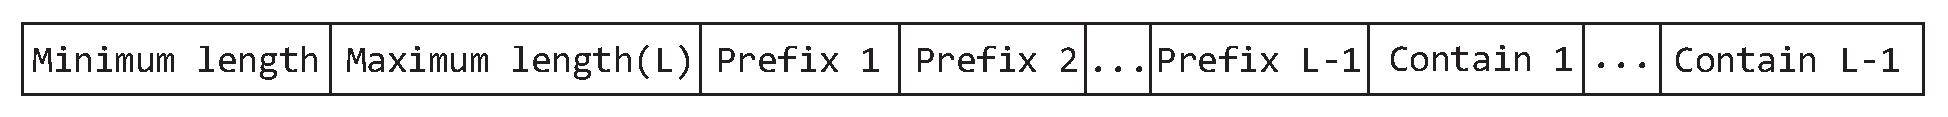
\includegraphics[width=\linewidth]{images/constraint.eps}
\caption{Constraints involving Strings.}
\label{fig:constraint}
\end{figure}

\tool\ leverages a hybrid approach to collect all possible constraints and thus
generates a high quality patch to repair the program. A constraint on a string
object is defined as a set of permissible values that can uniquely define the
string. \tool\ uses a simple constraint set that includes minimum and maximum
length, along with set of permissible prefixes and substrings, as shown in
Figure~\ref{fig:constraint}.

\begin{algorithm}[t]
\scriptsize
\DontPrintSemicolon
\KwData{Control flow graph $CFG$ for program $P$}
\KwResult{Patched program $\hat{P}$}
\Begin
{
 \For{$\forall$ node $N \in CFG$}
 {
  Statement $S$ in node $N$\;
  \If{$S$ conntaints \code{String} API call}
  {
  	$str \longleftarrow$ \code{String} reference on $S$\;
  	\If{$S$ can throw \code{RuntimeException}}
  	{
  		Exception class $EC \longleftarrow$ \code{RuntimeException} of
$S$\;
  		$CES_{str} \longleftarrow$ all conditional statement in $P$ on
$str$;
  		$CS_{str} \longleftarrow$ output of
  		Algorithm~\ref{algo:constraintCollection}$(CES_{str})$ \;
  		\If{$str$ have sufficient constraints in $CS_{str}$}
  		{
  			$str \longleftarrow$ output of
Algorithm~\ref{algo:constraint}$(CS_{str})$\;
  		} \lElse   		{
  			$str \longleftarrow$ output of
  			Algorithm~\ref{algo:stringPatchParametr}$(S)$\;
  		}
  		Instrument ~\ref{algo:constraintCollection}$(CES_{str})$ in $P$
for dynamic
  		constraint collection\;
  		Instrument ~\ref{algo:constraint}$(CS_{str})$ in $P$ for dynamic
  		constraint evaluation\;
  	}
  }
 }
}
\caption{Patching strategy for \code{String} objects}
 \label{algo:patchingStrategy}
\end{algorithm}

The hybrid approach has a static component that makes a forward pass over the
program to collect declarative constraints on string objects, such as their
length or prefix, etc. \tool\ invokes the dynamic component if there are
conflicting constraints such that the constraint set cannot be evaluated. In
such scenarios \tool\ (i) generates a patch that itself dynamically collects
constraint information, (ii) augments it with the previously collected static
constraint details, and (iii) evaluates these constraints on the fly to generate
repaired \code{String} objects, which do not cause the program to throw runtime
exceptions. Algorithm~\ref{algo:patchingStrategy} briefly describes this hybrid
approach.

\begin{algorithm}[t]
\scriptsize
\DontPrintSemicolon
\KwData{Set of conditional statement on string $str$}
\KwResult{Constraint set $CS_{str}$}
\Begin
{
  \For{Conditional statement$ \leftarrow i$, $\forall i \in CS_{str}$}
  {
   $i \Rightarrow str\ *\ OP$ \code{/*where $*$ is the binary operator*/}\\
   \lIf{$*$ is $==$} {\\
   \mytab $maxlength_{str} \longleftarrow OP$\\
   \mytab $minlength_{str} \longleftarrow OP$
   } \lElseIf {$*$ is $\textgreater$ {\bf AND} $*$ is $\ge$} {
    $minlength_{str} \longleftarrow OP$
   } \lElseIf {$*$ is $\textless$ {\bf AND} $*$ is $\le$} {
    $maxlength_{str} \longleftarrow OP$
   } \lElseIf {$*$ is Prefix Check} {
    $PrefixSet_{str} \cup OP$
   } \lElseIf {$*$ is Contains Check} {
    $ContainSet_{str} \cup OP$
   }
  }
}
\caption{Constraint collection for \code{String} objects}
\label{algo:constraintCollection}
\end{algorithm}

\myparagraph{Static constraint collection}: \tool's static constraint collection
phase identifies and stores all declarative constraints. Specifically, \tool\
iterates over all program code and analyzes conditional statements involving
string objects to determine the possible constraints that the object must
satisfy if the control flow should take the \textit{preferred} branch of the
conditional. We define the \textit{preferred} branch as one that does not throw
exceptions or error conditions, like \code{System.err.print()}. In other words,
\tool\ only considers the conditional expressions in the branches that do not
involve any exceptions or error paths.

Algorithm~\ref{algo:constraintCollection} lists the steps to collect the
constraints 

\myparagraph{Dynamic constraint collection}

\begin{algorithm}[t]
\scriptsize
\DontPrintSemicolon
\KwData{String object $Str$ and constraint set $CS$.}
\KwResult{String object $Str$ such that $\forall i \in CS$, $Str$ satisfies $i$}
\Begin {
    $CS_{Str} \longleftarrow$ Get the constraint set for $Str$\;
    $MinLength \longleftarrow CS_{Str}[0]$\;
    $MaxLength \longleftarrow CS_{Str}[1]$\;
    $PrefixSet_{Str} \longleftarrow CS_{Str}[2 \rightarrow MaxLength + 1]$\;
    $ContainSet_{Str} \longleftarrow CS_{Str}[MaxLength +2  \rightarrow
2*MaxLength + 1]$\;

    \For{$C \in PrefixSet_{Str}$} {
        \If{$C$ is Empty} {
            continue\;
        }
        $PrefixLength \longleftarrow$ {\bf LENGTH OF} $C$\;
        \If{$PrefixLength$ is Maximum $\in PrefixSet_{Str}$} {
            Use $C$ to construct $Str$\;
        }
    }

    \For{$C \in ContainSet_{Str}$} {
        \If{$C$ is Empty {\bf OR} $C \in Str$} {
            continue\;
        }
        $Str \leftarrow Str$ {\bf APPEND} $C$\;
    }
    return $Str$\;
}
\caption{String object constraint evaluation}
\label{algo:constraint}
\end{algorithm}

\begin{mylist}

 \item \textbf{Object repairing}

 \item \textbf{API parameter tweaking}

\begin{algorithm}[t]
\scriptsize
\DontPrintSemicolon
\KwData{String object $Str$ and index set $IS$ which contains ${i}$ or ${i,j}$.}
\KwResult{Repaired index set containing ${Ri}$ or ${Ri,Rj}$ based on input $IS$}
\Begin {
    $Length \longleftarrow$ length of $Str$\;
    \If{$Length == 0$} {
        $Ri, Rj \longleftarrow 0$\;
    } \Else {
        \If{$i \textgreater j$} {
            $Ri \longleftarrow j - 1$;
        }
        \If{$i \textgreater Lengrh$ \bf{OR} $j \textgreater Lengrh$} {
            $Ri \longleftarrow Length - 1$ or $Rj \longleftarrow Length - 1$
based on condition\;
        }
        \If{$i \textless 0$ \bf{OR} $j \textless 0h$} {
            $Ri \longleftarrow 0$ or $Rj \longleftarrow 0$ based on
condition\;
        }
    }
}
\caption{String patching based on parameters passed}
\label{algo:stringPatchParameter}
\end{algorithm}

\end{mylist}

\subsubsection{Code generation}
\label{sec:tool:stage2:generation}

\subsection{Instrumentation}
\label{sec:tool:stage3}

try-catch
catch ladder

We have find such statements which can potentially throw \code{RuntimeException}
and we put them in try-catch block and place appropriate patch inside the catch
block based on the appropriate exception type to make sure
the exception is suppressed and the operation we performed
in patch maintains the safe bound.

\ignore{
\paragraph{Identifying Program Statements.} We perform static taint analysis
to identify sensitive data which are leaving the system via database, network
stream, file stream or console. Providing patches to the
statements that manipulate this data would be undesirable, since
activation of the patches in case failures may allow altered sensitive data to
eventually
reach users. Hence, we only mark those program statements which do
not manipulate these data.

\paragraph{Noninvasive Patching.} In case a runtime exception that is thrown
by a statement as a result of a failure is already caught and handled in a
program,
we skip that statement from patching to avoid interfering with the results. Such
statements are identified by analyzing call-graphs and ensuring that no caller
method
in the call-chain handles the exception or its superclass. By embedding the
patches inside
\texttt{catch} blocks, we ensure that they do not get activated during normal
program execution.

\paragraph{Patch Generation.} We first perform an
intra-procedural static analysis
to identify constraints on the string objects under consideration. By
identifying
the type of exceptions that can be thrown in case of a failure, we
develop patches that
regenerate string objects by tweaking \java\ \code{String} API used in
the statements to regenerate legal string objects and by trying to solve the
constraints. In the latter case,
we evaluate the constraints statically if complete information is available at
the compilation-time. Otherwise, the analysis automatically generates
code that performs dynamic analysis to solve the constraints, and then
inserts this code in the generated patches.

\paragraph{Optimizing Instrumentation.} We perform reaching definitions
analysis to skip marked statements
if the string variables that are contained in the statements are already
patched, and the variables
are not redefined along any path that originates from the patched statement.
This analysis reduces
instrumentation points in a program.

\paragraph{Patch Precision.} The precision of a program patch is improved,
firstly, by targeting only strings
for patching which allows us to develop more specialized patches, secondly, by
patching programs very
close to the points of potential failures which avoids unnecessary patching of
other
unaffected variables and their potential
side effects, thirdly, by analyzing the types of exceptions that can be thrown
which
provides valuable insights into
origins of failures, and finally, by considering all the constraints
on the strings. This would result
in a program behavior closed to the intended one in case of a failure.

\paragraph{Reduced Overhead.} The side-effect of non-invasive patches is that
they do not interfere during
normal execution which results in no runtime overhead. Even when they get
activated in case of failures,
they still cause negligible overhead since we perform no analysis during runtime
except if required resolve the dynamic constraints.
As our study reveals~\xref{sec:evaluation} the constraints are typically few and
simple, making
the dynamic analysis light-weight.
}

